\documentclass[conference]{IEEEtran}
\IEEEoverridecommandlockouts

\usepackage{amsmath,amssymb,amsfonts}
\usepackage{booktabs}
\usepackage{array}
\usepackage{multirow}
\usepackage{graphicx}
\graphicspath{{figures/imported/}{manuscript/figures/imported/}}
\usepackage{cite}
\usepackage{url}
\usepackage{balance}

\newcommand{\BSC}{\ensuremath{\mathrm{BSC}_{6}}}
\newcommand{\R}{\mathbb{R}}
\newcommand{\Ind}{\mathbf{1}}

\title{On the Edge of Stability: Spiking Reservoir State-Space Encoding of Affective EEG}

\author{
\IEEEauthorblockN{Andrew A. Lane\IEEEauthorrefmark{1}, Wendy Tang\IEEEauthorrefmark{1}, and Brady D. Nelson\IEEEauthorrefmark{2}}
\IEEEauthorblockA{\IEEEauthorrefmark{1}Department of Electrical and Computer Engineering, Stony Brook University, Stony Brook, NY, USA}
\IEEEauthorblockA{\IEEEauthorrefmark{2}Department of Psychology, Stony Brook University, Stony Brook, NY, USA}
}

\begin{document}
\maketitle

\begin{abstract}
Affective EEG event-related potentials (ERPs) are noisy, subject-dependent measurements of evoked neural dynamics, and robustness rankings can depend as much on the evaluation protocol as on the representation being evaluated. We compare four affective-ERP representations under subject-grouped validation with subject-level uncertainty: spectral band-power, ERP-window amplitudes, a fixed leaky integrate-and-fire reservoir summarized by a six-bin spike-count (\BSC{}) embedding and operated near its measured edge of stability ($\rho^\ast\approx0.82$; removing the recurrence costs $0.049$ balanced accuracy, BA, $95\%$ CI $[-0.098,-0.002]$), and a trained EEGNet, with electrode removal, amplitude noise, and temporal jitter applied to the raw signal identically for every encoder. Two channel-dropout artifacts are quantified. First, raw retention favors near-chance models: the reservoir has $100\%$ raw retention at $30\%$ dropout largely because its clean BA is only $0.487$, close to the $1/3$ chance floor. Second, zero-imputation of dropped channels creates out-of-distribution standardized values for non-centered features, and we show algebraically that it is not invariant to an information-preserving re-centering. Across $10$--$50\%$ dropout and mean, $k$NN, and spatial fills, in-distribution imputation raises non-centered encoders by up to $0.13$ BA, while the reservoir's zero-centered embedding changes little; at $30\%$ dropout, zero-fill halves the measured lead of ERP-window features over the reservoir ($+0.05$ versus $+0.09$ to $+0.11$ BA). For EEGNet, loss to electrode removal is more than halved by training-time channel-dropout augmentation, which raises BA at $30\%$ removal from $0.660$ to $0.703$ while preserving clean performance ($0.731$). The imputation effect also appears on DEAP, where the measured robustness of the same band-power features changes by up to $0.11$ BA under the imputation rule alone. These results support a simple reporting standard for EEG robustness studies: report absolute accuracy with subject-level uncertainty alongside retention, specify and vary the imputation rule, and state whether trained models used perturbation augmentation.
\end{abstract}


\begin{IEEEkeywords}
EEG, event-related potentials, spiking neural networks, reservoir computing, affective computing, neuromorphic computing, ARSPI-Net.
\end{IEEEkeywords}

\section{Introduction}
Electroencephalographic event-related potentials (ERPs) provide millisecond-scale measurements of evoked neural dynamics, but the recorded waveform is a noisy, low-dimensional, and subject-dependent projection of an unobserved neural process \cite{makeig2002dynamic,blankertz2011singletrial}. A representation may separate affective conditions under one protocol while preserving little usable structure after amplitude noise, temporal misalignment, or channel loss.

Endpoint accuracy alone also says little about what a representation preserves, which matters for spiking encodings. Fixed recurrent reservoirs and spiking networks provide nonlinear temporal expansions \cite{maass2002real,lukosevicius2009reservoir}, but EEG/ERP studies often treat them primarily as classifiers \cite{gong2023sglnet,craik2019deep}, and their spike-count features are rarely examined as perturbation-sensitive temporal measurements. How affective-ERP reservoir encodings change under perturbation remains underreported, even though preprocessing, acquisition, and electrode-loss choices can materially change EEG representation performance \cite{delpup2025preprocessing,chiang2023depression,guo2025mma}.

This paper evaluates whether channel-dropout robustness rankings for affective-ERP representations are stable under reasonable changes to the scoring protocol. We compare spectral band-power, ERP-window amplitudes, a fixed leaky integrate-and-fire (LIF) reservoir summarized by six post-onset spike-count bins (\BSC{}) and compressed for a linear readout, and a trained EEGNet. The reservoir is not treated as a proposed winner; it is used as a fixed reference whose embedding is nearly zero-centered and whose dynamics are not retrained under perturbation. The contributions are:
\begin{enumerate}
    \item A subject-grouped robustness comparison of affective-ERP representations under electrode removal, amplitude noise, and temporal jitter applied identically to every encoder's input, with subject-level confidence intervals and a permutation null (Secs.~\ref{sec:clean}, \ref{sec:rawsignal}; Tables~\ref{tab:clean}--\ref{tab:rawsignal}).
    \item Quantification of two protocol artifacts in channel-dropout evaluation: raw-retention inflation near the chance floor, and zero-imputation bias for non-centered features. The imputation effect is also tested on DEAP (Secs.~\ref{sec:confound}, \ref{sec:perturb}, \ref{sec:deap}).
    \item Paired subject-level evidence that zero-imputation halves the measured lead of ERP-window features over the reservoir, while channel-dropout augmentation more than halves the trained EEGNet's loss to electrode removal (Fig.~\ref{fig:impute}, Tables~\ref{tab:dropconf}, \ref{tab:rawsignal}).
    \item A fixed-reservoir reference analysis: a spectral-radius sweep with a no-recurrence ablation and a measured order parameter placing the transition at $\rho^\ast\approx0.82$ (Fig.~\ref{fig:resdyn}), and a single-bin ablation separating the state-space expansion from temporal bin granularity (Eq.~\eqref{eq:operator}).
\end{enumerate}
Clinical labels and affective categories define the task structure; the representations and their invariances under perturbation are the object of study.

\section{Related Work}
\label{sec:related}
ERP/EEG analysis commonly uses time-window amplitudes and latencies, Hjorth \cite{hjorth1970eeg} and wavelet/spectral descriptors \cite{subasi2007eeg}, and linear models \cite{blankertz2011singletrial}. These features are interpretable in relation to known ERP components such as the P300 and late positive potential \cite{makeig2002dynamic}, but can miss nonlinear temporal interactions. Reservoir computing offers a complementary approach: a high-dimensional recurrent dynamical system maps the input to a state trajectory that can be read out by a simple classifier \cite{maass2002real,jaeger2001echo,jaeger2004harnessing,lukosevicius2009reservoir}. Spiking liquid-state machines add event-based timing and count structure \cite{diehl2015unsupervised,roy2019towards}. Reservoir computation is often reported to peak near the transition between ordered and chaotic dynamics, located by how far a small state perturbation spreads \cite{bertschinger2004realtime,legenstein2007edge}; for a thresholded spiking reservoir, whose recurrence enters only through binary spikes, that transition need not coincide with the $\rho=1$ echo-state heuristic for rate reservoirs \cite{jaeger2001echo}. When the recurrent dynamics are fixed, the reservoir can be analyzed as a measurement operator rather than only as a classifier.

Spiking and deep networks are now widely applied to EEG \cite{gong2023sglnet,lawhern2018eegnet,craik2019deep}. Much of this literature still emphasizes endpoint accuracy, while preprocessing and acquisition choices receive less systematic treatment \cite{delpup2025preprocessing,kornblith2019similarity}. Neuromorphic reservoir features for affective EEG were introduced in prior ARSPI-Net work \cite{lane2023arspi,lane2024arspi}; here we establish their perturbation and invariance properties and identify two scoring artifacts that distort robustness comparisons.

Dynamic spatial filtering addresses missing or corrupted channels with a learned channel-attention front end \cite{banville2022dsf}, and channel-dropout or amplitude-noise augmentation are standard ways to harden trained models \cite{rommel2022augment}. A recent EEG foundation-model benchmark reports that no single model is most robust to all perturbations and that apparent channel-dropout fragility can depend on whether dropped channels are removed or zero-padded \cite{sirca2026beyond}. More broadly, missing-data handling in neuroimaging spans a spectrum from constant fills and spherical-spline interpolation of absent electrodes~\cite{perrin1989spherical}, through learned imputation and learned spatial filtering~\cite{banville2022dsf}, to conditional generative synthesis of entire missing modalities with ViT-GAN and latent-diffusion models~\cite{bi2024graymatters,hu2025gmldm}. The four fills we study sit at the simple, non-learned end of that spectrum. We build on the benchmark's point by separating two scoring effects, raw-retention inflation for low-accuracy representations and zero-imputation bias for non-centered fixed features, using the training-free, nearly fill-invariant reservoir as the reference case.

\section{Methods}
\label{sec:methods}
\subsection{ERP Observation Model}
Let $X_s^{(c)}\in\R^{C\times T}$ denote the trial-averaged ERP observation for subject $s$ and affective condition $c$, with $C$ electrodes (channels) and $T$ temporal samples. We treat $X_s^{(c)}$ as a noisy observation of an unobserved neural state trajectory:
\begin{equation}\label{eq:obs}
    \xi_{t+1}=f_\theta(\xi_t,u_t)+\eta_t,\qquad
    x_t=H\xi_t+\epsilon_t,
\end{equation}
where $\xi_t$ is the latent neural state, $H$ is a measurement operator induced by scalp observation, and $\epsilon_t$ captures measurement and preprocessing noise; the perturbations below act on this model (Sec.~\ref{sec:perturb}).

\subsection{Spiking Reservoir Encoding}
For each electrode trace, the signal is passed through a fixed LIF reservoir of $256$ neurons with recurrent weights $W$ scaled to spectral radius $\rho=0.9$ (near the measured edge of stability; Fig.~\ref{fig:resdyn}d), input weights $W_{\mathrm{in}}$, leak parameter $\beta=0.05$, and firing threshold $\vartheta=0.5$:
\begin{align}
    v_{t} &= \big[(1-\beta)\,(1-z_{t-1})\odot v_{t-1} + W z_{t-1} + W_{\mathrm{in}}x_t\big]_+, \\
    z_{t} &= \Ind[v_{t}\geq \vartheta],
\end{align}
where $v_t$ is the membrane state, $z_t$ is the binary spike vector, $[\cdot]_+$ is rectification at zero, and the factor $(1-z_{t-1})$ resets every unit that spiked at the previous step. $W_{\mathrm{in}}$ and $W$ are drawn once from a Xavier-uniform law (seed $42$); the reservoir is fixed, and only the readout is trained. To test whether the recurrent dynamics matter, the same reservoir is rescaled to $\rho\in\{0,0.3,0.6,0.9,1.2,1.5\}$ with every other parameter fixed ($\rho=0$ removes the recurrence, leaving a feedforward LIF layer). A label-free order parameter locates the dynamical transition by damage spreading~\cite{bertschinger2004realtime}: two copies receive the same electrode drive, one unit's spike is flipped at the start of the analysis window, and the mean normalized Hamming distance between the copies' spike vectors over the rest of the window shows whether the flip dies out (ordered) or spreads (irregular); $\rho^\ast$ is the half-maximum crossing of this curve over $\rho\in[0,2]$, interpolated on a grid of step $0.1$.

Activity is summarized by six equal temporal bins over the window $t\in[10,70)$ in sample units; with stimulus onset at sample $51$ (Sec.~\ref{sec:data}), this spans about $-160$ to $+73$~ms around onset. For reservoir unit $j$ and bin $k$, the binned spike-count code is $b_{j,k}=\sum_{t\in\mathcal{B}_k} z_j(t)$, $k=1,\ldots,6$. Per-electrode spike-bin features are compressed to $64$ principal components and concatenated across the $34$ channels into a trial-level reservoir representation $E_s^{(c)}\in\R^{2176}$. The encoding is a fixed composition of a nonlinear temporal map, spike-count binning, and the unsupervised projection:
\begin{equation}\label{eq:operator}
E=\phi_{\mathrm{PCA}}\!\big([b_1,\dots,b_6]\big)=\Phi(X),
\end{equation}
so $E=\Phi(X)$ is a fixed, label-free representation. The PCA basis is fitted, unsupervised, on the training subjects of each fold only; fitting it once over all subjects (transductive with respect to subject inclusion) is reported as a sensitivity check in Sec.~\ref{sec:clean}. A single-bin control (BSC$_1$, total spike count in the window) uses the identical pipeline. The window lies mostly before onset and excludes the later components the ERP-window baseline sees; because every epoch is z-scored over its full length, pre-stimulus samples also carry an offset set by the post-stimulus signal, so we do not attribute the reservoir's accuracy to a specific evoked component.

\begin{figure*}[t]
\centering
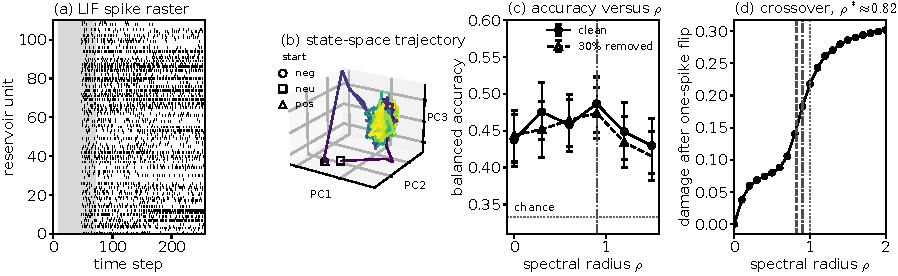
\includegraphics[width=0.76\textwidth]{fig_reservoir_dyn.pdf}
\caption{The fixed LIF reservoir as a dynamical system, linked to accuracy. (a)~Spike raster (units $0$--$109$ of $256$) for one condition (shaded $=$ the $t\in[10,70)$ window, about $-160$ to $+73$~ms around onset at step $51$). (b)~Population state-space trajectory (first three principal components of the membrane state), from epoch start (dark) to end (light), for the three conditions; the trajectories largely overlap, consistent with the modest clean separability. (c)~Subject-level BA ($95\%$ CI) versus spectral radius $\rho$, clean and with $30\%$ of electrodes removed; $\rho=0$ removes the recurrence, and the dash-dot line marks the pre-specified $\rho=0.9$. (d)~Damage-spreading order parameter versus $\rho$; shading separates the ordered and irregular regimes at the measured transition $\rho^\ast\approx0.82$; dash-dot $=$ $\rho=0.9$, dotted $=$ the echo-state heuristic $\rho=1$.}
\label{fig:resdyn}
\end{figure*}



\subsection{Baselines and Readout}
Two classical baselines are evaluated under the same subject-grouped protocol. The band-power baseline (A0) uses Welch band power in five bands ($1$--$4$, $4$--$8$, $8$--$13$, $13$--$30$, $30$--$45$~Hz) per channel ($5\times34=170$ dimensions). The ERP-window baseline (A0$_e$) uses mean amplitude in three fixed windows, about $-120$--$0$~ms (pre-stimulus baseline), $50$--$250$~ms (early components), and $250$--$600$~ms (P300 and late positive potential) relative to onset, per channel ($3 \times 34 = 102$ dimensions). The band-power, ERP-window, and reservoir representations use a balanced L2-regularized logistic readout to test separability without a high-capacity classifier.

As a trained deep baseline we evaluate EEGNet-8,2~\cite{lawhern2018eegnet} on the raw $34\times256$ ERP signal under the identical subject-grouped folds, trained per fold (Adam, $80$ epochs) with train-only per-channel standardization, with and without augmentation by random channel dropout and additive noise.

\subsection{Perturbation Diagnostics}
Two experiments are separated. The feature-coordinate experiment (Sec.~\ref{sec:perturb}) suppresses a dropped channel's feature block after extraction and refills it by one of four rules; it isolates the fill convention and the coordinate origin, and applies to the fixed encoders. The signal-level experiment (Sec.~\ref{sec:rawsignal}) corrupts the test subjects' raw signal before any feature extraction, identically for every encoder including EEGNet (same draws in each fold; training on the clean signal): removal of $10$, $30$, or $50\%$ of the electrodes, white noise at $5$~dB SNR per channel, and an alignment shift of up to $\pm50$~ms, with all features recomputed from the corrupted signal. In Eq.~\eqref{eq:obs}, noise augments $\epsilon_t$, removal zeroes rows of $H$, and jitter shifts the sampling index of $x_t$. Performance is balanced accuracy (BA); Table~\ref{tab:clean} also reports macro-F1 and macro one-vs-rest ROC-AUC.

\subsection{Retention Scores and Two Confounds}
\label{sec:confound}
We report two robustness summaries. \emph{Raw retention} is the ratio of perturbed to clean BA. Because BA is bounded below by chance ($c=1/3$ for three balanced classes), raw retention can overstate the stability of representations whose clean performance is already close to chance. We therefore also report \emph{above-chance retention}, $(\mathrm{BA}_{\mathrm{pert}}-c)/(\mathrm{BA}_{\mathrm{clean}}-c)$.

Channel dropout also requires a fill rule for the dropped channel's features. The common zero-fill convention is not neutral after train-only standardization: a zero-valued feature becomes $-\mu/\sigma$, which can be out of distribution for non-centered features. Train-mean imputation maps the dropped feature to the standardized origin. We compare zero-fill with train-mean imputation, then add two in-distribution checks: train-fitted $k$-nearest-neighbor imputation ($k{=}10$) and a within-sample spatial fill using the mean of retained channels. EEGNet has no intermediate feature vector, so it enters only the signal-level experiment, with and without augmented training.

\emph{Non-invariance of zero-imputation robustness.} For a feature with training mean $\mu$ and standard deviation $\sigma$, an imputed value $v$ enters the readout as $(v-\mu)/\sigma$, so zero- and mean-imputation differ by a fixed shift,
\begin{equation}\label{eq:noninv}
\frac{0-\mu}{\sigma}-\frac{\mu-\mu}{\sigma}=-\frac{\mu}{\sigma}.
\end{equation}
Train-only standardization leaves clean readout performance unchanged under a constant re-centering $x\mapsto x-b$, but the zero-imputation input shifts by $b/\sigma$. Thus zero-imputation robustness is not invariant to an information-preserving re-centering; the two fills coincide if and only if $\mu=0$ on the dropped coordinates, which is why a mean-centered embedding such as PCA provides a useful reference point: averaged over features and training folds, $|\mu|/\sigma$ is $0.06$ for the reservoir, against $0.75$ for ERP-window and $1.20$ for band-power.

\section{Experimental Protocol}
\subsection{Dataset and Task}
\label{sec:data}
The experiments use trial-averaged affective ERP data from the Stress, Health, and the Psychophysiology of Emotion (SHAPE) project~\cite{shape}, collected by the Laboratory for Clinical Affective Neuroscience at Stony Brook University, with 211 subjects after exclusion of one anomalous subject record. Each subject contributes three affective conditions (negative, neutral, pleasant), yielding 633 subject-condition observations. Each recorded epoch ($34$ scalp channels at $1024$~Hz, $1.2$~s, baseline-corrected over the $200$~ms pre-stimulus interval) is analyzed as every fourth of its first $1024$ samples: $256$ samples at $256$~Hz spanning $-200$ to $+800$~ms around stimulus onset (onset at sample $51$), z-scored per channel within each epoch; the grand averages show the expected late-positive-potential enhancement for emotional over neutral stimuli (Fig.~\ref{fig:erp}). Subject-level data are maintained in a restricted research environment; only aggregate, de-identified results are reported.

\begin{figure*}[t]
\centering
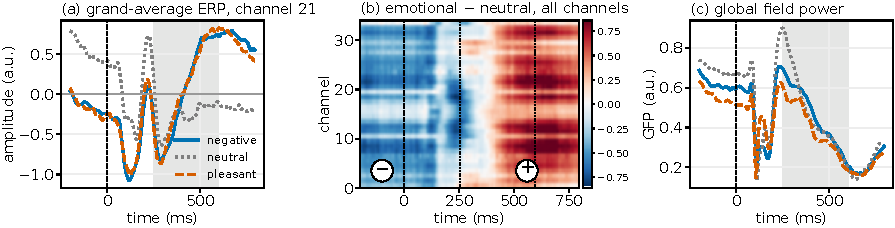
\includegraphics[width=0.56\textwidth]{fig_erp.pdf}
\caption{Trial-averaged affective ERP data (SHAPE cohort; grand averages over 211 subjects). (a)~Grand-average waveforms per condition at the most affect-discriminative channel; time $0$ $=$ stimulus onset (dashed), shaded $=$ the late ERP-window feature ($250$--$600$~ms). (b)~Spatiotemporal map of the emotional-minus-neutral difference across all $34$ channels (dotted $=$ the same window; $-$/$+$ mark the sign), showing the sustained LPP enhancement. (c)~Global field power per condition.}
\label{fig:erp}
\end{figure*}

\subsection{Validation}
All results are computed under a single protocol: StratifiedGroupKFold (5 folds, seeds $42$--$46$), train-only standardization, and a balanced L2 logistic readout; observations from the same subject never span train and test, and EEGNet is trained on the same folds. Uncertainty is estimated at the level of the subject, not the fold: for each representation we average the out-of-fold class probabilities of every observation across the five repeated partitions, then form $95\%$ confidence intervals (CIs) from $4000$ resamples of the $211$ subjects with replacement, keeping a resampled subject's three observations together; macro one-vs-rest AUC uses the same pooled probabilities. Comparisons between encoders, fills, or conditions are paired differences under the same subject resampling. Because the partitions are pooled into one prediction per observation before resampling, the dependence among the $25$ overlapping fold estimates does not enter the intervals, and no test treats folds as independent samples. Chance is calibrated by a within-subject label-permutation null ($20$ permutations).

\section{Results}
\subsection{Clean Classification and Controls}
\label{sec:clean}
Table~\ref{tab:clean} reports clean three-class performance. The trained EEGNet is the most accurate representation (BA $0.731$, $95\%$ CI $[0.701,0.763]$); among the fixed encoders, ERP-window features lead (A0$_e$, $0.629$), above band-power (A0, $0.494$) and the reservoir embedding (A1, $0.487$), whose subject-level intervals overlap. A within-subject label-permutation null gives mean BA $0.33$ to $0.34$ (SD at most $0.023$, maximum $0.39$) for every fixed encoder, so each encodes genuine signal (more than five null SDs above chance) while its clean separability remains modest.


\begin{table}[t]
\caption{Clean three-class performance with subject-level bootstrap $95\%$ CIs, macro-F1, and macro one-vs-rest ROC-AUC from the pooled out-of-fold probabilities. Chance is $1/3$ (AUC $0.5$); permutation-null BA is $0.33$ to $0.34$.}
\label{tab:clean}
\centering
\small
\setlength{\tabcolsep}{2pt}
\begin{tabular}{llccc}
\toprule
Cfg & Features & BA [95\% CI] & F1 & AUC \\
\midrule
D0 & EEGNet (raw, trained) & $0.731$ [$0.701$, $0.763$] & -- & -- \\
A0$_e$ & ERP-window (102) & $0.629$ [$0.597$, $0.660$] & $0.629$ & $0.799$ \\
A0 & Band-power (170) & $0.494$ [$0.460$, $0.528$] & $0.492$ & $0.682$ \\
A1 & Reservoir \BSC{} (2176) & $0.487$ [$0.447$, $0.523$] & $0.485$ & $0.658$ \\
-- & Reservoir BSC$_1$ (2176) & $0.487$ [$0.450$, $0.523$] & -- & -- \\
\bottomrule
\end{tabular}
\end{table}

\emph{Temporal-binning ablation.} The single-bin total-count code (BSC$_1$) matches \BSC{}: the paired difference \BSC{} minus BSC$_1$ is $+0.001$ BA ($95\%$ CI $[-0.044,+0.047]$) clean and $-0.001$ ($[-0.046,+0.041]$) with $30\%$ of electrodes removed, so the reservoir's accuracy comes from the fixed state-space expansion, not temporal bin granularity; we claim no temporal-coding benefit for \BSC{}.

\emph{Spectral radius and recurrent dynamics.} The recurrent dynamics contribute: relative to the pre-specified $\rho=0.9$, the feedforward layer ($\rho=0$) loses $0.049$ BA ($95\%$ CI $[-0.098,-0.002]$), and the strongly irregular $\rho=1.5$ loses $0.057$ ($[-0.106,-0.011]$; $-0.058$, $[-0.103,-0.016]$, with $30\%$ of electrodes removed; Fig.~\ref{fig:resdyn}c). Between $\rho=0.3$ and $1.2$ the differences from $\rho=0.9$ are within noise, as is the $\rho=0$ contrast under $30\%$ removal ($-0.030$, $[-0.074,+0.016]$), so the optimum is broad. The order parameter rises steadily, with its largest increment between $\rho=0.8$ and $0.9$, and saturates above $\rho\approx1.2$; its half-maximum crossing places the transition at $\rho^\ast\approx0.82$, below the echo-state heuristic $\rho=1$ (Fig.~\ref{fig:resdyn}d), and the mean firing rate doubles across it ($0.06$ at $\rho=0.6$, $0.12$ at $\rho=0.9$). The pre-specified operating point thus lies next to the measured edge of the ordered regime, inside the broad optimum.

\emph{Transduction and component controls.} Fitting the PCA basis on all subjects (transductive) gives BA $0.485$ $[0.447,0.521]$, against $0.487$, and $\{16,32,64,128\}$ components give $0.477$--$0.507$, inside the $64$-component interval, so neither accounts for the reported results.

\subsection{Two Confounds in Channel-Dropout Robustness}
\label{sec:perturb}
Channel dropout is where the reported conclusion depends on the scoring convention (Table~\ref{tab:dropconf}, Fig.~\ref{fig:impute}).

\emph{Accuracy-floor effect.} With zero-imputation, raw retention ranks the reservoir first at $30\%$ dropout: its BA does not move (retention $100\%$, against $85\%$ for ERP-window). That interpretation is misleading because the reservoir's clean BA ($0.487$) is close to the $1/3$ chance floor, leaving less above-chance performance to lose. Above-chance retention corrects the floor, but its denominator is only about $0.15$ for the reservoir, so it is unstable near chance and can exceed one; we therefore treat absolute BA and paired subject-level differences as primary, with retention ratios as secondary diagnostics.

\emph{Zero-imputation effect.} Zeroing a dropped channel's features and then standardizing maps them to $-\mu/\sigma$, an out-of-distribution value for a non-centered feature; train-mean imputation instead maps it to the standardized origin. At $30\%$ dropout, this raises band-power from $0.417$ to $0.472$ and ERP-window features from $0.536$ to $0.578$, while the reservoir does not change ($0.487$ under both fills), consistent with its PCA-centered embedding. ERP-window features lead the reservoir under every fill, but the fill sets the size of the lead: the paired difference ERP-window minus reservoir is $+0.049$ BA ($95\%$ CI $[+0.003,+0.095]$) under zero-fill and $+0.092$ to $+0.107$ under the three in-distribution fills, whose CIs all lie above $+0.04$. Zero-imputation thus halves the measured advantage of the strongest fixed encoder, because only the non-centered encoder's score moves with the constant.

\emph{Generality.} The mean-minus-zero gaps at $30\%$ dropout are $+0.042$ ($[+0.011,+0.074]$) for ERP-window, $+0.055$ ($[+0.024,+0.087]$) for band-power, and $-0.000$ ($[-0.022,+0.022]$) for the reservoir, ordered as the non-centeredness in Eq.~\eqref{eq:noninv}. Across $10$--$50\%$ dropout the reservoir's two constant-fill scores agree within $0.016$~BA and no CI excludes zero, whereas the gap of the non-centered encoders varies with the rate and is significant for band-power at $20$ and $30\%$ and for ERP-window at $30\%$ (Fig.~\ref{fig:impute}a). $k$NN fill differs in kind (Fig.~\ref{fig:impute}b): it replaces the dropped block by an average over ten training neighbors, adding content rather than moving the origin, and at $40$ and $50\%$ it significantly raises every encoder, ERP-window most ($+0.13$~BA at $50\%$, $[+0.09,+0.16]$). At $30\%$, $k$NN/spatial fills give $0.610$/$0.589$ (ERP-window), $0.483$/$0.488$ (band-power), and $0.507$/$0.482$ (reservoir).

\begin{table}[t]
\caption{Channel dropout at $30\%$: naive and corrected evaluation. ``Zero'' and ``Mean'' denote zero- and train-mean imputation of dropped channels; for EEGNet, a raw-signal model, ``Zero'' is signal-level removal of $30\%$ of the electrodes (Table~\ref{tab:rawsignal}). Raw-ret. is $\mathrm{BA}_{\mathrm{zero}}/\mathrm{BA}_{\mathrm{clean}}$; AC-ret. is above-chance retention under mean-imputation (removal for EEGNet); ``+aug.'' denotes train-time augmentation. Per-cell $95\%$ CIs are $\pm0.03$ to $\pm0.04$.}
\label{tab:dropconf}
\centering
\small
\setlength{\tabcolsep}{3.5pt}
\begin{tabular}{lccccc}
\toprule
Representation & Clean & Zero & Mean & raw-ret. & AC-ret. \\
\midrule
EEGNet & $0.731$ & $0.660$ & -- & $90\%$ & $82\%$ \\
\quad +\,aug. & $0.731$ & $0.703$ & -- & $96\%$ & $93\%$ \\
ERP-window & $0.629$ & $0.536$ & $0.578$ & $85\%$ & $83\%$ \\
Band-power & $0.494$ & $0.417$ & $0.472$ & $84\%$ & $86\%$ \\
Reservoir & $0.487$ & $0.487$ & $0.487$ & $100\%$ & $100\%$ \\
\bottomrule
\end{tabular}
\end{table}

\begin{figure}[t]
\centering
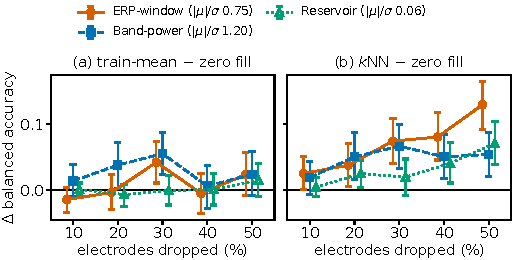
\includegraphics[width=0.86\columnwidth]{fig_impute_subj.pdf}
\caption{How much the fill rule alone moves channel-dropout accuracy: paired subject-level change in BA relative to zero-fill, with $95\%$ CIs, versus the share of electrodes dropped. (a)~Train-mean fill, which differs from zero-fill only by the shift of Eq.~\eqref{eq:noninv}; the legend gives each encoder's mean $|\mu|/\sigma$. (b)~$k$NN fill, which replaces the dropped block by an average of ten training neighbors and so changes its content.}
\label{fig:impute}
\end{figure}

\subsection{Signal-Level Perturbations}
\label{sec:rawsignal}
The signal-level experiment corrupts the recorded signal itself, identically for every encoder (Table~\ref{tab:rawsignal}). A removed electrode contributes zero band-power and zero ERP amplitude, so for these two encoders removal is exactly zero-fill and their removal rows equal the zero-fill scores of Sec.~\ref{sec:perturb}; for the reservoir, a silent electrode yields a zero spike-count block that projects to the negative of the projected training mean rather than to the PCA origin, so the shift of Eq.~\eqref{eq:noninv} reappears before the projection.

Three results stand out. First, ERP-window features remain the most accurate fixed encoder under every condition; their paired lead over the reservoir is $+0.06$ to $+0.14$~BA, every CI excluding zero. Second, the reservoir holds its accuracy through $30\%$ removal (loss $0.013$, $95\%$ CI $[-0.014,+0.041]$) but falls to $0.393$ at $50\%$, close to chance (loss $0.093$, $[+0.055,+0.131]$), so its fill invariance is a property of its feature space, not robustness to missing electrodes. Third, $5$~dB noise costs band-power $0.059$~BA ($[+0.019,+0.098]$) while ERP-window and the reservoir stay within noise of their clean scores, and $\pm50$~ms jitter moves no fixed encoder, consistent with the wide ERP windows and the single-bin control of Sec.~\ref{sec:clean}.

\emph{Training effect.} EEGNet ingests the same corrupted signal and is the most accurate encoder in every condition (paired lead over ERP-window $+0.08$ to $+0.20$, every CI excluding zero); unaugmented, it loses $0.071$~BA at $30\%$ removal and $0.144$ at $50\%$, close to the ERP-window losses ($0.093$ and $0.155$). Re-training with channel-dropout and amplitude-noise augmentation leaves clean accuracy unchanged (paired difference $-0.000$, $[-0.025,+0.022]$) and cuts these losses by more than half, to $0.028$ and $0.062$: the augmented network is ahead by $+0.043$ ($[+0.009,+0.077]$) at $30\%$ and $+0.082$ ($[+0.049,+0.115]$) at $50\%$, and neither variant loses more than $0.024$~BA to noise or jitter. For this trained baseline, dropout robustness is therefore strongly affected by the training procedure, not only by the architecture (Fig.~\ref{fig:deapaug}b).

\begin{table}[t]
\caption{Signal-level perturbations: subject-level BA with every representation recomputed from the corrupted test signal (same draws for all encoders; training on clean data, EEGNet also with augmentation). Per-cell $95\%$ CIs are $\pm0.03$ to $\pm0.04$; chance is $1/3$.}
\label{tab:rawsignal}
\centering
\small
\setlength{\tabcolsep}{3pt}
\begin{tabular}{lccccc}
\toprule
Condition & Band-pow. & ERP-win. & Reserv. & EEGNet & +aug. \\
\midrule
Clean & $0.494$ & $0.629$ & $0.487$ & $0.731$ & $0.731$ \\
$10\%$ removed & $0.476$ & $0.602$ & $0.469$ & $0.719$ & $0.722$ \\
$30\%$ removed & $0.417$ & $0.536$ & $0.474$ & $0.660$ & $0.703$ \\
$50\%$ removed & $0.450$ & $0.474$ & $0.393$ & $0.588$ & $0.670$ \\
Noise $5$~dB & $0.436$ & $0.619$ & $0.479$ & $0.738$ & $0.727$ \\
Jitter $\pm50$~ms & $0.496$ & $0.626$ & $0.493$ & $0.719$ & $0.708$ \\
\bottomrule
\end{tabular}
\end{table}

\subsection{External Replication on an Independent Affective Dataset}
\label{sec:deap}
To test whether the imputation effect is specific to SHAPE, we evaluate band-power features on DEAP~\cite{koelstra2012deap}, an independent affective EEG dataset (32 subjects, 40 trials each), on a binary valence task under the standard within-subject protocol (per-subject stratified $5$-fold; DEAP band-power is at chance cross-subject). The same pattern appears, larger than in SHAPE (Fig.~\ref{fig:deapaug}a). At $30\%$ dropout, band-power scores BA $0.540$ under zero-imputation ($95\%$ CI $[0.528,0.552]$) but $0.621$ $[0.591,0.648]$ under mean and $0.638$ $[0.607,0.668]$ under $k$NN imputation, with CIs from resampling the $32$ subjects' mean BA. With clean BA $0.639$, zero-imputation indicates a $0.10$ BA loss and $k$NN imputation almost none: for the same features on a second dataset, task, and montage, the imputation convention alone moves measured robustness by up to $0.11$ BA.

\begin{figure}[t]
\centering
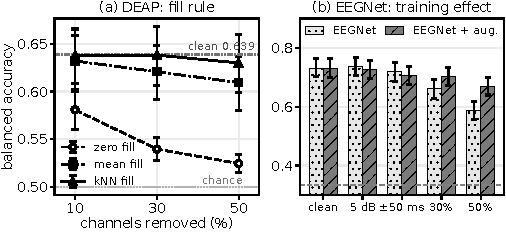
\includegraphics[width=0.86\columnwidth]{fig_deap_aug.pdf}
\caption{(a)~External check on DEAP~\cite{koelstra2012deap} (32 subjects, within-subject binary valence, band-power; clean BA $0.639$; CIs from resampling subjects). Channel-dropout BA changes substantially with the imputation rule. (b)~EEGNet without and with channel-dropout and noise augmentation under the signal-level conditions of Table~\ref{tab:rawsignal} (subject-level $95\%$ CIs): augmentation leaves clean accuracy unchanged, moves noise and jitter accuracy by at most $0.011$, and cuts the loss to electrode removal by more than half.}
\label{fig:deapaug}
\end{figure}

\section{Discussion}
The main result is methodological. Channel-dropout robustness estimates change under two common reporting choices: raw retention can favor models close to the chance floor, and zero-imputation can penalize non-centered features after standardization; for trained models, augmentation is a third factor. The zero-fill effect agrees with the benchmark finding that channel-dropout fragility depends on whether dropped channels are removed or zero-padded~\cite{sirca2026beyond}, and Eq.~\eqref{eq:noninv} gives its mechanism. After accounting for these choices, the fixed reservoir should not be described as the most channel-robust encoder: ERP-window features lead it under every fill at $30\%$ dropout and under every signal-level condition, zero-imputation halves that lead, and the augmented EEGNet is the most accurate and the strongest dropout baseline here. The reservoir remains useful as a fixed reference because its centered embedding changes little across imputation rules, making the imputation artifact visible in the other encoders, but its invariance belongs to its feature space and does not survive signal-level removal of half the electrodes. Its dynamics still matter: removing the recurrence or driving it into the irregular regime lowers accuracy, and the operating point lies next to the measured edge of the ordered regime, in line with edge-of-chaos results for other reservoirs~\cite{bertschinger2004realtime,legenstein2007edge}.

Learned and generative imputation sit further along the same spectrum (Sec.~\ref{sec:related}); if non-learned fills already move measured accuracy by up to $0.13$~BA and halve an encoder difference, the fill model of a learned imputer is part of the measured result and should be reported with it. These results suggest a minimal reporting standard for EEG robustness studies: report absolute accuracy with subject-level uncertainty alongside raw and above-chance retention, state the channel-fill rule, test at least one in-distribution fill, and report trained-model results with and without perturbation augmentation. None requires a new model, but each changes how the comparison is interpreted.

\textbf{Limitations.} The primary cohort is a single trial-averaged affective-ERP dataset. The imputation effect follows from the standardization algebra in Eq.~\eqref{eq:noninv} and is observed across three imputation rules, five dropout rates, and the independent DEAP check, but paradigm-matched multi-cohort ERP validation would strengthen it. EEGNet is trained with one fixed recipe, without a hyperparameter search, and the spectral-radius sweep uses a single draw of the reservoir weights. Adversarial attacks and montage shifts are not evaluated; graph topology and structure--function coupling are outside the scope of this paper.

\section{Conclusion}
Channel-dropout robustness rankings for affective-ERP representations depend on the scoring protocol. Raw retention can overstate robustness near the chance floor, zero-imputation can distort non-centered features after standardization, and trained models need their augmentation state made explicit. Here, zero-imputation halves the measured lead of the strongest fixed encoder, the spiking reservoir operated near its measured edge of stability makes these effects visible without being the most accurate encoder, and the imputation effect replicates on DEAP. Paradigm-matched, multi-cohort ERP data are the next test of this reporting protocol.

\textbf{Ethics.} The SHAPE study was collected by the Stony Brook University Laboratory for Clinical Affective Neuroscience under that laboratory's Institutional Review Board oversight. DEAP is a publicly released dataset governed by its original collection protocol~\cite{koelstra2012deap}. \textbf{Data Availability.} For the SHAPE dataset, contact the Laboratory for Clinical Affective Neuroscience at Stony Brook University~\cite{shape}; DEAP is public~\cite{koelstra2012deap}.

\IEEEtriggeratref{15}
\begin{thebibliography}{99}

\bibitem{maass2002real}
W. Maass, T. Natschl\"ager, and H. Markram, ``Real-time computing without stable states: A new framework for neural computation based on perturbations,'' \emph{Neural Computation}, vol. 14, no. 11, pp. 2531--2560, 2002.

\bibitem{jaeger2001echo}
H. Jaeger, ``The echo state approach to analysing and training recurrent neural networks,'' German National Research Center for Information Technology, GMD Report 148, 2001.

\bibitem{jaeger2004harnessing}
H. Jaeger and H. Haas, ``Harnessing nonlinearity: Predicting chaotic systems and saving energy in wireless communication,'' \emph{Science}, vol. 304, no. 5667, pp. 78--80, 2004.

\bibitem{lukosevicius2009reservoir}
M. Luko\v{s}evi\v{c}ius and H. Jaeger, ``Reservoir computing approaches to recurrent neural network training,'' \emph{Computer Science Review}, vol. 3, no. 3, pp. 127--149, 2009.

\bibitem{bertschinger2004realtime}
N. Bertschinger and T. Natschl\"ager, ``Real-time computation at the edge of chaos in recurrent neural networks,'' \emph{Neural Computation}, vol. 16, no. 7, pp. 1413--1436, 2004.

\bibitem{legenstein2007edge}
R. Legenstein and W. Maass, ``Edge of chaos and prediction of computational performance for neural circuit models,'' \emph{Neural Networks}, vol. 20, no. 3, pp. 323--334, 2007.

\bibitem{diehl2015unsupervised}
P. U. Diehl and M. Cook, ``Unsupervised learning of digit recognition using spike-timing-dependent plasticity,'' \emph{Frontiers in Computational Neuroscience}, vol. 9, p. 99, 2015.

\bibitem{roy2019towards}
K. Roy, A. Jaiswal, and P. Panda, ``Towards spike-based machine intelligence with neuromorphic computing,'' \emph{Nature}, vol. 575, pp. 607--617, 2019.

\bibitem{lane2023arspi}
A. Lane, W. Tang, and B. Nelson, ``Towards ARSPI-Net: Development of an efficient hybrid deep learning framework,'' in \emph{Proc. IEEE Long Island Systems, Applications and Technology Conf. (LISAT)}, Old Westbury, NY, USA, 2023, pp. 1--8.

\bibitem{lane2024arspi}
A. Lane, W. Tang, and B. Nelson, ``Towards ARSPI-Net: Advancing EEG feature extraction with neuromorphic algorithms,'' in \emph{Proc. IEEE Long Island Systems, Applications and Technology Conf. (LISAT)}, Holtsville, NY, USA, 2024, pp. 1--8.

\bibitem{gong2023sglnet}
P. Gong, P. Wang, Y. Zhou, and D. Zhang, ``A spiking neural network with adaptive graph convolution and LSTM for EEG-based brain-computer interfaces,'' \emph{IEEE Trans. Neural Syst. Rehabil. Eng.}, vol. 31, pp. 1440--1450, 2023.

\bibitem{hjorth1970eeg}
B. Hjorth, ``EEG analysis based on time domain properties,'' \emph{Electroencephalography and Clinical Neurophysiology}, vol. 29, no. 3, pp. 306--310, 1970.

\bibitem{subasi2007eeg}
A. Subasi, ``EEG signal classification using wavelet feature extraction and a mixture of expert model,'' \emph{Expert Systems with Applications}, vol. 32, no. 4, pp. 1084--1093, 2007.

\bibitem{makeig2002dynamic}
S. Makeig, M. Westerfield, T.-P. Jung, S. Enghoff, J. Townsend, E. Courchesne, and T. J. Sejnowski, ``Dynamic brain sources of visual evoked responses,'' \emph{Science}, vol. 295, no. 5555, pp. 690--694, 2002.

\bibitem{blankertz2011singletrial}
B. Blankertz, S. Lemm, M. Treder, S. Haufe, and K.-R. M\"uller, ``Single-trial analysis and classification of ERP components: a tutorial,'' \emph{NeuroImage}, vol. 56, no. 2, pp. 814--825, 2011.

\bibitem{lawhern2018eegnet}
V. J. Lawhern, A. J. Solon, N. R. Waytowich, S. M. Gordon, C. P. Hung, and B. J. Lance, ``EEGNet: A compact convolutional neural network for EEG-based brain-computer interfaces,'' \emph{Journal of Neural Engineering}, vol. 15, no. 5, 056013, 2018.

\bibitem{craik2019deep}
A. Craik, Y. He, and J. L. Contreras-Vidal, ``Deep learning for electroencephalogram (EEG) classification tasks: A review,'' \emph{Journal of Neural Engineering}, vol. 16, no. 3, 031001, 2019.

\bibitem{chiang2023depression}
H.-S. Chiang, M.-Y. Chen, and L.-S. Liao, ``Cognitive depression detection cyber-medical system based on EEG analysis and deep learning approaches,'' \emph{IEEE J. Biomed. Health Inform.}, vol. 27, no. 2, pp. 608--616, 2023.

\bibitem{guo2025mma}
Y. Guo, K. Yang, and Y. Wu, ``A multi-modality attention network for driver fatigue detection based on frontal EEG, EDA and PPG signals,'' \emph{IEEE J. Biomed. Health Inform.}, vol. 29, no. 6, pp. 4009--4022, 2025.

\bibitem{delpup2025preprocessing}
F. Del Pup, A. Zanola, L. F. Tshimanga, A. Bertoldo, and M. Atzori, ``The more, the better? Evaluating the role of EEG preprocessing for deep learning applications,'' \emph{IEEE Trans. Neural Syst. Rehabil. Eng.}, vol. 33, pp. 1061--1070, 2025.

\bibitem{kornblith2019similarity}
S. Kornblith, M. Norouzi, H. Lee, and G. Hinton, ``Similarity of neural network representations revisited,'' in \emph{Proc. Int. Conf. Machine Learning}, 2019, pp. 3519--3529.

\bibitem{sirca2026beyond}
U. \v{S}irca, M. Alimardani, S. Zafeiriou, and K. Barmpas, ``Beyond accuracy: Robustness, interpretability and expressiveness of EEG foundation models,'' \emph{arXiv:2605.17562}, 2026.

\bibitem{banville2022dsf}
H. Banville, S. U. N. Wood, C. Aimone, D.-A. Engemann, and A. Gramfort, ``Robust learning from corrupted EEG with dynamic spatial filtering,'' \emph{NeuroImage}, vol. 251, 118994, 2022.

\bibitem{rommel2022augment}
C. Rommel, J. Paillard, T. Moreau, and A. Gramfort, ``Data augmentation for learning predictive models on EEG: A systematic comparison,'' \emph{Journal of Neural Engineering}, vol. 19, no. 6, 066020, 2022.

\bibitem{perrin1989spherical}
F. Perrin, J. Pernier, O. Bertrand, and J. F. Echallier, ``Spherical splines for scalp potential and current density mapping,'' \emph{Electroencephalography and Clinical Neurophysiology}, vol. 72, no. 2, pp. 184--187, 1989.

\bibitem{bi2024graymatters}
Y. Bi, A. Abrol, S. Jia, J. Sui, and V. D. Calhoun, ``Gray matters: ViT-GAN framework for identifying schizophrenia biomarkers linking structural MRI and functional network connectivity,'' \emph{NeuroImage}, vol. 297, 120674, 2024.

\bibitem{hu2025gmldm}
X. Hu, J. Yang, S. Jia, Y. Bi, and V. D. Calhoun, ``GM-LDM: Latent diffusion model for brain biomarker identification through functional data-driven gray matter synthesis,'' arXiv:2506.12719, 2025.

\bibitem{koelstra2012deap}
S. Koelstra \emph{et al.}, ``DEAP: A database for emotion analysis using physiological signals,'' \emph{IEEE Trans. Affective Computing}, vol. 3, no. 1, pp. 18--31, 2012.

\bibitem{shape}
Laboratory for Clinical Affective Neuroscience, ``The Stress, Health, and the Psychophysiology of Emotion (SHAPE) project,'' Stony Brook University, Stony Brook, NY, USA. [Online]. Available: \url{https://lab-can.com}

\end{thebibliography}

\end{document}